%% LyX 2.0.0 created this file.  For more info, see http://www.lyx.org/.
%% Do not edit unless you really know what you are doing.
\documentclass[english]{article}
\usepackage{beramono}
\usepackage[T1]{fontenc}
\usepackage[latin9]{inputenc}
\usepackage{listings}
\usepackage{float}
\usepackage{graphicx}

\makeatletter
%%%%%%%%%%%%%%%%%%%%%%%%%%%%%% User specified LaTeX commands.
\usepackage[usenames,dvipsnames]{color}

\makeatother

\usepackage{babel}
\begin{document}

\title{RL Homework 2}


\author{Chris Swetenham (s1149322)}


\date{April 2, 2012}

\maketitle

\section{MDP}

Similar to the previous assignment, we operate in a 3 by 4 grid world
surrounded by walls with no internal obstacles. Actions are movement
in the 4 cardinal directions. The start state is in one corner and
the goal state is one of the center states (state 7 in the standard
numbering). We formulate this as an MDP with a state for each coordinate
on the grid, represented by a single integer. We calculate possible
state transitions from the actions. We make the goal state a terminal
state. The reward is 0 when we are in the goal state, -1 otherwise.
We use a deterministic policy.

\medskip{}


\begin{figure}[H]


\centering{}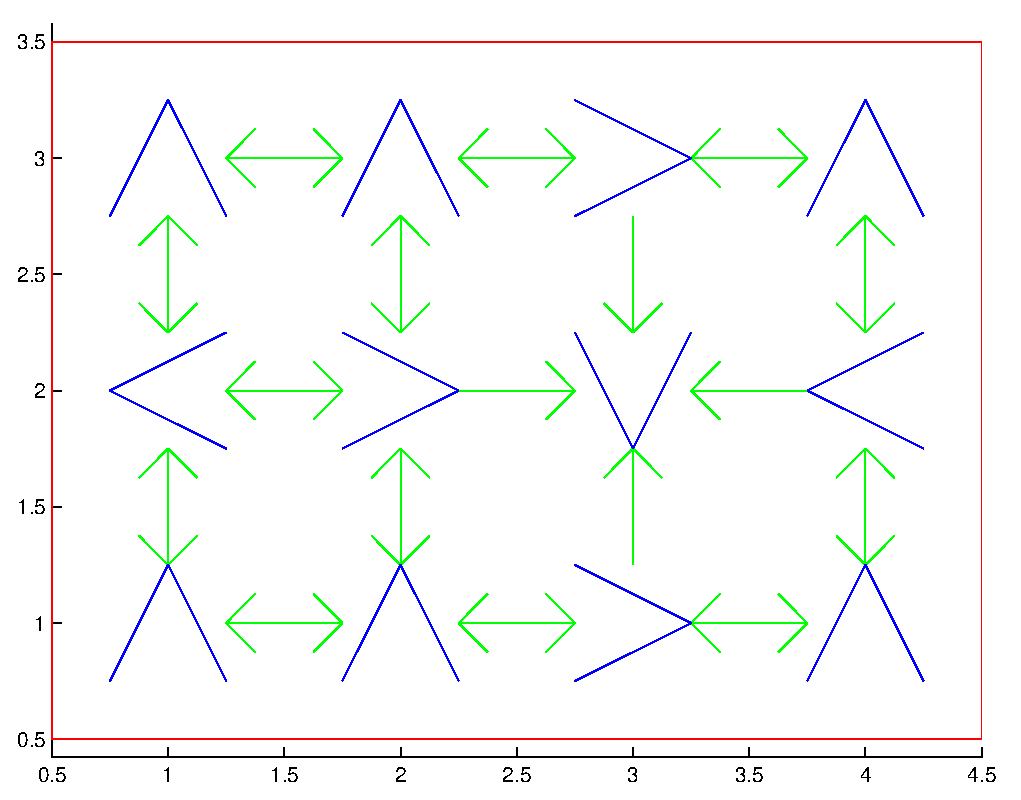
\includegraphics[width=0.5\textwidth]{StartingPolicy}\caption{Random Policy and State Transitions}
\end{figure}


We use the value iteration code from last assignment. We have also
modified it to return the Q-function directly which will be used later.
The value iteration procedure converges rapidly after 4 iterations,
giving the following value function and policy:

\begin{figure}[H]
\centering{}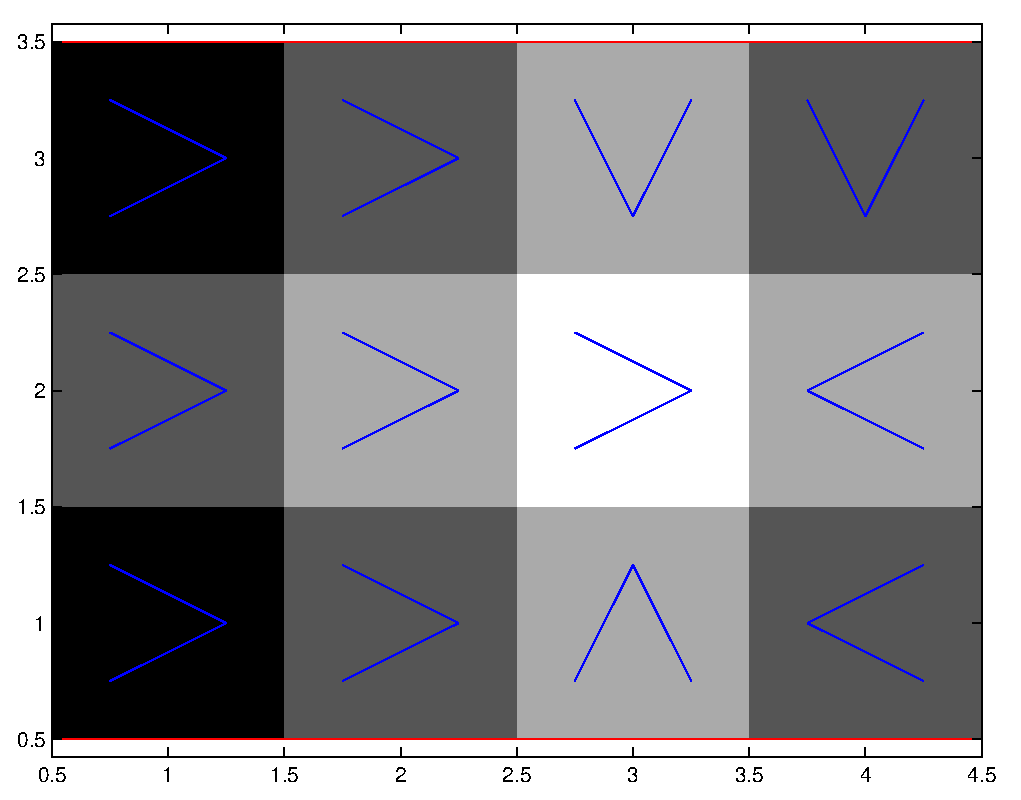
\includegraphics[width=0.5\textwidth]{ValueIteration}\caption{Optimal policy from value iteration}
\end{figure}


\medskip{}


\lstinputlisting[basicstyle={\scriptsize\ttfamily},breaklines=true,caption={part1.m},captionpos=b,commentstyle={\color{OliveGreen}},frame=tb,language=Matlab]{part1.m}


\section{Bayes Filter}

We now wish to formulate a Bayes Filter for localisation starting
from an uncertain state (maintaining deterministic state transitions).
We will evaluate this using a policy which chooses random actions
with equal probability, and the goal state is not taken into account.
The only signal available is a bump sensor which is triggered if the
robot bumps into a wall. In the usual formulation of the Bayes Filter,
the signal is a function of the current state, but here it is a function
of the state transition. We implement a version of the Bayes Filter
where the signal is a function of the previous state and the action
taken. We could have instead chosen to augment the state with an extra
bit to indicate the bumper status in the last transition, but this
seems like a less elegant formulation and it is desirable to avoid
needlessly increasing the number of states.

\medskip{}


\lstinputlisting[basicstyle={\scriptsize\ttfamily},breaklines=true,caption={bayesFilter.m},captionpos=b,commentstyle={\color{OliveGreen}},frame=tb,language=Matlab]{bayesFilter.m}

In our test run, the belief converges to one corner of the grid after
just 4 steps. The belief state is only reduced when some of the possible
states could have run into the wall and some would not have run into
the wall, under the latest action.

\begin{figure}[H]
\centering{}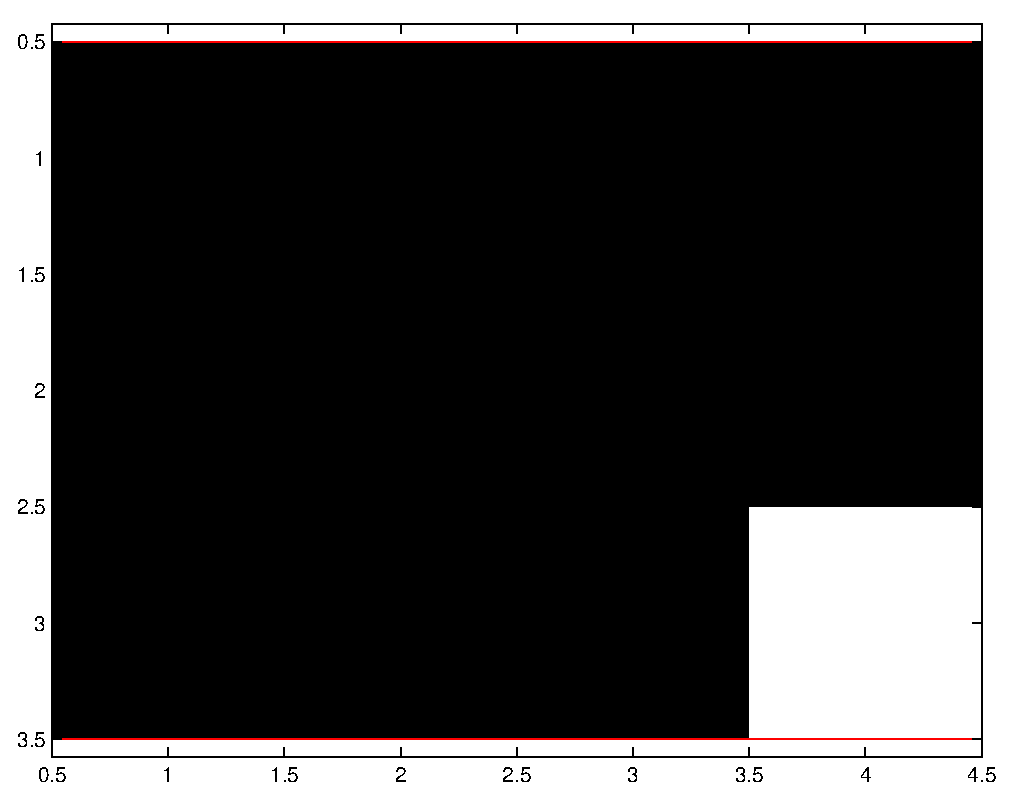
\includegraphics[width=0.5\textwidth]{BayesFilter}\caption{Converged belief from Bayes Filter}
\end{figure}


\medskip{}


\lstinputlisting[basicstyle={\scriptsize\ttfamily},breaklines=true,caption={part2.m},captionpos=b,commentstyle={\color{OliveGreen}},frame=tb,language=Matlab]{part2.m}


\section{QMDP}

We now combine the code from the previous sections in order to implement
QMDP. The initial state is unknown, but we compute the optimal value
function of the underlying MDP and then pick the optimal action according
to our belief and the value function.

As implied by the problem formulation we change the state transition
table for the QMDP run so that the goal state is no longer absorbing,
and instead terminate an episode when the belief has converged and
the robot is in the goal state.

We observe that the resulting process often does not converge. Trying
all possible starting states, we find that it converges only starting
from states 3 and 4, converging in 5 and 4 states respectively. From
other states, it will end up in a belief state where it will never
take an action that further constrains its belief state. Shown here
is the result after 100 iterations starting from state 12:

\begin{figure}[H]
\centering{}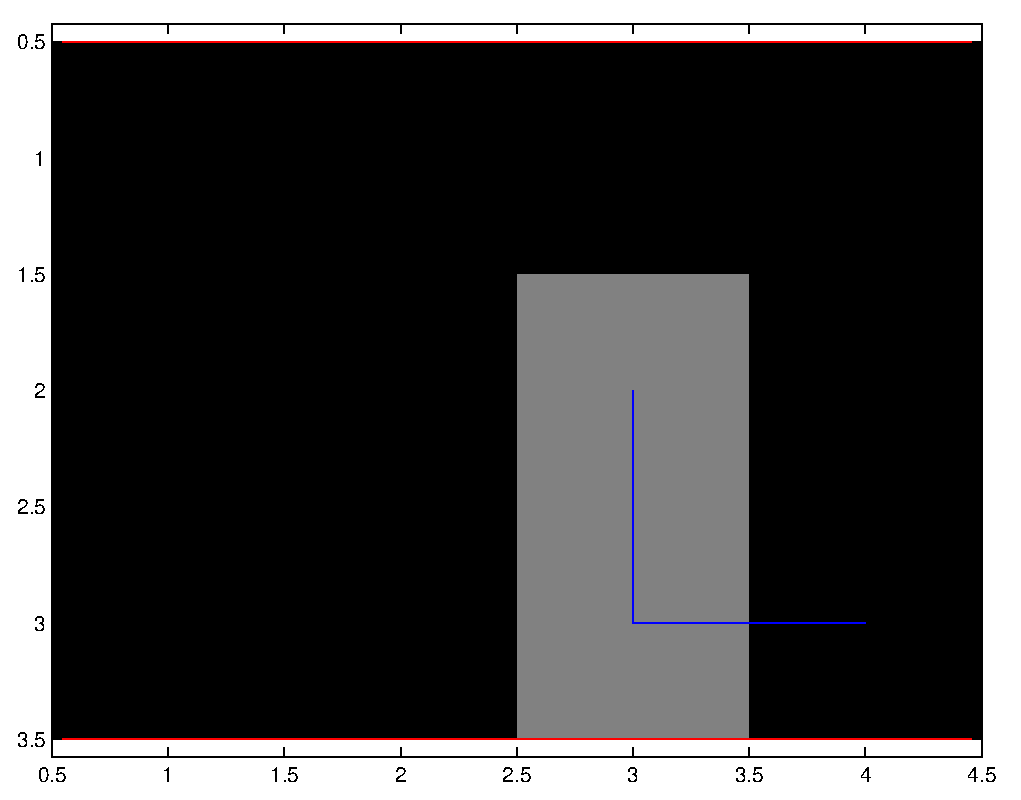
\includegraphics[width=0.5\textwidth]{QMDP-12}\caption{Non-convergence, starting from state 12}
\end{figure}


The non-converging situations have 2 or 4 possible states and hover
around the goal state without ever taking an action that might bump
into the wall and thereby reduce the belief state.

\medskip{}


\lstinputlisting[basicstyle={\scriptsize\ttfamily},breaklines=true,caption={part3.m},captionpos=b,commentstyle={\color{OliveGreen}},frame=tb,language=Matlab]{part3.m}


\section{Discussion}

We investigated making the policy of the QMDP algorithm non-deterministic
among the maximal-value choices, but this does not help in cases such
as the one in Figure 4. It is a fundamental limitation of QMDP that
it does not reason about future belief states when selecting an action.

In this toy environment, the actions and observations are deterministic,
so one simple way to fix the policy would be to first run right until
a bump, then down until a bump, thereby collapsing the belief state
in both dimensions; and then driving straight for the goal.

If the goal signal were made available to the bayes filter as an additional
input, it could localise the goal state correctly; but this would
often not correspond to a realistic situation in the real world.

We could try using an epsilon-greedy policy, although this would not
reliably produce a sequence of actions that reduce our belief state
in general.

We could also solve the full POMDP problem in this setting, using
point-based value iteration over the 12-dimensional belief state;
obviously this would be more computationally expensive but it is the
'correct' solution.


\section*{Appendix A - Additional Code}

\medskip{}
\lstinputlisting[basicstyle={\scriptsize\ttfamily},breaklines=true,caption={writeFigureEPS.m},captionpos=b,commentstyle={\color{OliveGreen}},frame=tb,language=Matlab]{writeFigureEPS.m}
\end{document}
